% arara: xelatex
% arara: bibtex
% arara: xelatex
% arara: xelatex

% Pattern Languages of Programs Conference 2023 October 22-25, 2023

% Original timeline:

% June 2         Shepherding begins
%% - We'll know if we have a shepherd
% June 30        Deadline focus group / workshop proposals
% August 7       Second draft due for review
% August 15      Notification of acceptance
% September 18   Conference versions due
% October 1      Conference registration ends
% October 22     Patterns Bootcamp
% October 23-25  PLoP Conference Days

% January 29, 2024 Proceeding version due

% Created 2021-11-16 Tue 16:22
% Intended LaTeX compiler: xelatex
\RequirePackage[prologue,table]{xcolor}
\documentclass[acmlarge,timestamp]{acmart}

%%%
\usepackage[many]{tcolorbox}
\usepackage{varwidth}
\usepackage{environ}
\usepackage{xparse}

\newlength{\bubblewidth}
\AtBeginDocument{\setlength{\bubblewidth}{.75\textwidth}}
\definecolor{bubblegreen}{rgb}{0.67, 0.9, 0.93}
\definecolor{bubblegray}{RGB}{241,240,240}

\newcommand{\bubble}[4]{%
  \tcbox[
    colback=#1,
    colframe=#1,
    #2,
  ]{\color{#3}\begin{varwidth}{\bubblewidth}#4\end{varwidth}}%
}

\ExplSyntaxOn
\seq_new:N \l__ooker_bubbles_seq
\tl_new:N \l__ooker_bubbles_first_tl
\tl_new:N \l__ooker_bubbles_last_tl

\NewEnviron{rightbubbles}
 {
  \raggedleft\sffamily
  \seq_set_split:NnV \l__ooker_bubbles_seq { \par } \BODY
  \int_compare:nTF { \seq_count:N \l__ooker_bubbles_seq < 2 }
   {
    \bubble{bubblegreen}{rounded~corners}{black}{\BODY}
   }
   {
    \seq_pop_left:NN \l__ooker_bubbles_seq \l__ooker_bubbles_first_tl
    \seq_pop_right:NN \l__ooker_bubbles_seq \l__ooker_bubbles_last_tl
    \bubble{bubblegreen}{sharp~corners=southeast}{black}{\l__ooker_bubbles_first_tl}\par
    \seq_map_inline:Nn \l__ooker_bubbles_seq
     {
      \bubble{bubblegreen}{sharp~corners=east}{black}{##1}\par
     }
    \bubble{bubblegreen}{sharp~corners=northeast}{black}{\l__ooker_bubbles_last_tl}\par
   }
 }
\NewEnviron{leftbubbles}
 {
  \raggedright\sffamily
  \seq_set_split:NnV \l__ooker_bubbles_seq { \par } \BODY
  \int_compare:nTF { \seq_count:N \l__ooker_bubbles_seq < 2 }
   {
    \bubble{bubblegray}{rounded~corners}{black}{\BODY}
   }
   {
    \seq_pop_left:NN \l__ooker_bubbles_seq \l__ooker_bubbles_first_tl
    \seq_pop_right:NN \l__ooker_bubbles_seq \l__ooker_bubbles_last_tl
    \bubble{bubblegray}{sharp~corners=southwest}{black}{\l__ooker_bubbles_first_tl}\par
    \seq_map_inline:Nn \l__ooker_bubbles_seq
     {
      \bubble{bubblegray}{sharp~corners=west}{black}{##1}\par
     }
    \bubble{bubblegray}{sharp~corners=northwest}{black}{\l__ooker_bubbles_last_tl}\par
   }
 }
\ExplSyntaxOff

%%%

\newfontfamily{\chess}[Color=red]{chess_merida_unicode.ttf}

\usepackage{xltxtra}
\usepackage{xelatexemoji}
\renewcommand{\xelatexemojipath}[1]{./svg/U#1.PDF}

\setcopyright{rightsretained}
\copyrightyear{2021}
\acmYear{2021}
\acmDOI{10.XXXX/XXXXXXX.XXXXXXX}

%% These commands are for a PROCEEDINGS abstract or paper.
\acmConference[PLoP'23]{PLoP'23: Pattern Languages of Programs 2023}{October 23--25, 2023}{HILLSIDE}
\acmBooktitle{PLoP'23, OCTOBER 5--7, HILLSIDE. Copyright 2023 is held by the author(s)}
\acmPrice{15.00}
\acmISBN{978-1-4503-XXXX-X/18/06}

%\usepackage[Latin,Greek,Emoticons]{ucharclasses}
\usepackage{graphicx}
\usepackage{grffile}
\usepackage{longtable}
\usepackage{wrapfig}
\usepackage{rotating}
\usepackage[normalem]{ulem}
%\usepackage{amsmath}
\usepackage{textcomp}
%\usepackage{amssymb}
\usepackage{capt-of}
\usepackage{hyperref}
\usepackage{fontspec}
\usepackage{mdframed}
\usepackage{afterpage}

\usepackage{booktabs}
%\usepackage[]{xcolor} %for use in color links
%\usepackage{colortbl}

\usepackage[pagewise]{lineno}
\renewcommand\thelinenumber{\color{red}\arabic{linenumber}}
\usepackage{xunicode}
\usepackage{natbib}
\usepackage{float}
\usepackage{xypic}
\usepackage{tikz}
\newcommand{\sensory}{(s)}
\newcommand{\cognitive}{(c)}
\newcommand{\motor}{(m)}
\newcommand*\circlednum[1]{\resizebox{1em}{!}{\tikz[baseline=(char.base)]{\node[shape=circle,draw,inner sep=2pt] (char) {#1};}}}
%\usepackage{amsmath, amssymb}
\def\t{\scriptstyle\triangle}
\def\T{\textstyle\blacktriangle}
\usepackage{placeins}
%\usepackage{starfont}
% \newfontfamily{\alch}{Alchemy}
\newfontfamily\emoji{DejaVu Sans}
%\newcommand{\Asclepius}{{\emoji\symbol{"2695}}}
%\newcommand{\Caduceus}{{\emoji\symbol{"2624}}}
\setmainfont{Libertinus Sans}
\newenvironment{echo}{}{}
\usepackage{enotez}
\renewcommand{\endnote}[1]{}
\newcommand{\ignorelink}[2][]{#2}
\newcommand{\markbf}[1]{\textsuperscript{\textbf{#1}}}
\setenotez{counter-format = alph, mark-cs = \markbf}
\DeclareInstance{enotez-list}{sverre}{paragraph}{heading={},notes-sep=\baselineskip,format=\normalsize\normalfont\raggedright\leftskip1.8em,number=\makebox[0pt][r]{#1.\ }\ignorespaces,}
\usepackage{epigraph}
\date{}
\title{Patterns of Patterns II: Discourse on Implementation}
\hypersetup{
 pdfauthor={Joseph Corneli et al.},
 pdftitle={Patterns of Patterns II},
 pdfkeywords={},
 pdfsubject={},
 pdfcreator={Emacs 30.0.50 (Org mode 9.6.1)}, 
 pdflang={English}}

\citestyle{acmauthoryear}
\let\cleardoublepage=\clearpage 
\begin{document}

\title{Patterns of Patterns II}

\author{Joseph Corneli}
\authornote{Corresponding author, jcorneli@brookes.ac.uk.}
\email{jcorneli@brookes.ac.uk}
\orcid{1234-5678-9012}
\affiliation{%
  \institution{Oxford Brookes University}
  \streetaddress{Gipsy Lane}
  \city{Oxford}
  \country{UK}
  \postcode{OX3 0BP}
}

\author{Noorah Alhasan}
\author{Leo Vivier}
\author{Alex Murphy}
\author{Raymond S. Puzio}
%\authornotemark[1]
\email{rsp@hyperreal.enterprises}
\affiliation{%
  \institution{Hyperreal Enterprises Ltd}
  \streetaddress{81 St Clement’s St}
  \city{Oxford}
  \country{UK}
  \postcode{OX4 1AW}}

\author{Abby Tabor}
\affiliation{%
  \institution{University of the West of England}
  \streetaddress{Faculty of Health and Applied Sciences (HAS), Frenchay Campus, Coldharbour Lane}
  \city{Bristol}
  \state{England}
  \country{UK}
  \postcode{BS16 1QY}}
\email{abby.tabor@uwe.ac.uk}

%% \author{Vitor Bruno}
%% \affiliation{%
%%   \institution{Milestone English}
%%   \streetaddress{Rua Trieste 170, ap2}
%%   \city{Palhoca}
%%   \state{SC}
%%   \country{Brazil}
%%   \postcode{88132-227}}
%% \email{chief@milestoneenglishcourse.com}

%% % \author{Paola Ricaurte}
%% % \affiliation{%
%% %   \institution{Tecnologico de Monterrey}
%% %   \streetaddress{Calle del Puente 222 Col. Ejidos de Huipulco, Tlalpan}
%% %   \city{Mexico City}
%% %   \country{Mexico}
%% % }
%% % \email{pricaurt@tec.mx}

\author{Sridevi Ayloo}
\affiliation{%
  \institution{New York City College of Technology}
  \streetaddress{300 Jay St}
  \city{Brooklyn}
  \postcode{11201}
  \country{USA}
}
\email{pricaurt@tec.mx}

\author{Charlotte Pierce}
\affiliation{%
  \institution{Pierce Press}
  \streetaddress{PO Box 206}
  \city{Arlington MA}
  \country{USA}
  \postcode{02476}
}
\email{charlotte.pierce@gmail.com}

\author{Charles J. Danoff}
\affiliation{%
  \institution{Mr Danoff’s Teaching Laboratory}
 \streetaddress{PO Box 802738}
 \city{Chicago}
 \state{IL}
  \country{USA}
  \postcode{60680}}
\email{contact@mr.danoff.org}

\author{Mary Tedeschi}
\author{Manvinder Singh}
\author{Kajol Khetan}
\affiliation{%
  \institution{Baruch College}
 \streetaddress{PO Box 802738}
 \city{New York}
 \state{NY}
  \country{USA}
  \postcode{60680}}
\email{mtedeschi@pace.edu}


%%
%% By default, the full list of authors will be used in the page
%% headers. Often, this list is too long, and will overlap
%% other information printed in the page headers. This command allows
%% the author to define a more concise list
%% of authors' names for this purpose.
\renewcommand{\shortauthors}{Corneli et al.}


% (1) Review the intention: what do we expect to learn or make together?

% - Joe: Wanted to walk through the PoP paper with Rebecca, in order to help solidify my own grasp of the concepts and get her feedback.
% - Rebecca: This topic sounded interesting when you mentioned it and I wanted to learn about Pop

% (2) Establish what is happening: what and how are we learning?

% - Indeed we did speed through the paper, Rebecca pointed out a few places where there was friction with the wording or concepts, like ``PEER-TO-PEER'' and also suggested Operational Research and Strategy as an appropriate topic; mentioned “improvisatory” style
% - Interruptions were welcomed!
% - Rebecca: was hesitant to interrupt the narrative
% - This is a bit different from usual IEAI style...

% (3) What are some different perspectives on what’s happening?

% - Joe: appreciate the time Rebecca has put into this a lot, and I also think this was a good way to present the paper
% - Rebecca: I think you assume knowledge in the presentation, and I think you need to assume the listener (if they aren’t in the area) that they don’t know anything.  It wouldn’t be patronising to explain the basic concepts.

% (4) What did we learn or change?

% - Talking to Karl, he would reconise one of the areas (probably) but not necessarily the other two.  Everyone is going to be new to some of these concepts.
% - This was great as a ``final edit'' — we will also be able to edit this paper until December
% - RR: is it your aim to automate?

% (5) What else should we change going forward?

% - Joe: if it would be helpful to RR, I’d certainly be happy to meet again about these ideas
% - Would this (patterns of patterns) to actually be useful for ethical AI?
% - E.g., rethink in the context of moral machines

%%
%% The abstract is a short summary of the work to be presented in the
%% article.
% distributed peer-to-peer networks
\begin{abstract}
We review how our earlier theorization of pattern methods fares in the
wild.  The “wild” here included a graduate school classroom in New
York, a workshop at a transdisciplinary conference in Arizona, a
nascent citizen science project in Bristol, and a professional
development day for a university in Oxford.  We encountered unexpected
challenges such as working with students in a HyFlex classroom,
getting conference attendees to feel comfortable evaluating the
conference they were presently attending, and adapting our plans on
the fly when leading workshops with surprising attendee responses.  We
describe and refine pattern specifications that will help other
practitioners of patterns in their own forays into the wild.
\end{abstract}

%%
%% The code below is generated by the tool at http://dl.acm.org/ccs.cfm.
%% Please copy and paste the code instead of the example below.
%%
\begin{CCSXML}
<ccs2012>
<concept>
<concept_id>10003456</concept_id>
<concept_desc>Social and professional topics</concept_desc>
<concept_significance>500</concept_significance>
</concept>
<concept>
<concept_id>10011007.10011074.10011075</concept_id>
<concept_desc>Software and its engineering~Designing software</concept_desc>
<concept_significance>300</concept_significance>
</concept>
<concept>
<concept_id>10011007.10011074.10011134.10003559</concept_id>
<concept_desc>Software and its engineering~Open source model</concept_desc>
<concept_significance>300</concept_significance>
</concept>
<concept>
<concept_id>10010405.10010481</concept_id>
<concept_desc>Applied computing~Operations research</concept_desc>
<concept_significance>300</concept_significance>
</concept>
<concept>
<concept_id>10010147.10010341</concept_id>
<concept_desc>Computing methodologies~Modeling and simulation</concept_desc>
<concept_significance>100</concept_significance>
</concept>
</ccs2012>
\end{CCSXML}

\ccsdesc[500]{Social and professional topics}
\ccsdesc[300]{Software and its engineering~Designing software}
\ccsdesc[300]{Software and its engineering~Open source model}
\ccsdesc[300]{Applied computing~Operations research}
\ccsdesc[100]{Computing methodologies~Modeling and simulation}


%%
%% Keywords. The author(s) should pick words that accurately describe
%% the work being presented. Separate the keywords with commas.
\keywords{Design Patterns, Pattern Languages, Action Reviews, Futures
Studies, Causal Layered Analysis, Emacs, Free Software, Peeragogy,
Climate Change, Innovation, Anticipation}

%\authorsaddresses{This command processes the author and affiliation and title This command processes the author and affiliation and title This command processes the author and affiliation and title This command processes the author and affiliation and title}

%%
%% This command processes the author and affiliation and title
%% information and builds the first part of the formatted document.
\maketitle


%\clearpage

\section{Introduction}
\label{sec:org195e8e3}
\label{Introduction}

%% ACTUAL START OF THE PAPER
%% {\color{red}
%% The previous installation in this series presented a high-level
%% methodological synthesis that aimed to get at the heart of what design
%% patterns are \cite{patterns-of-patterns-i}.  Here, we want to talk
%% about how we have implemented the methods described previously, and
%% give some reflections on where things are going next.  We will begin with a
%% recapitulation of the main points made in the earlier paper.  In
%% short, “Patterns of Patterns” encapsulated everything we had to say
%% about design patterns with \emph{one} overall pattern which operated
%% at a very high level.  Here, we elaborate many practical patterns
%% which expand on the same theme.  This fully-fledged collection of
%% patterns of patterns can help you organise your work with Design
%% Pattern Language methods.}

The previous installation in this series presented a high-level
methodological synthesis of three techniques from design, futures
studies, and learning management
in the form of a design pattern
called PLACARD \cite{patterns-of-patterns-i}.  We saw the PLACARD pattern as really getting to the heart of what design patterns are.
To back up this claim, we presented a theoretical analysis, and a case
study.  During the two years which have elapsed since then, we have
had opportunities to deploy and further develop these methods in
various contexts.  We will describe some of these applications in the
four cases studies below.  We have distilled this experience into a
collection of practical patterns which augment the earlier high-level
pattern.  This fully-fledged collection of patterns of patterns can
help you organise your work with Design Pattern Language methods.

% \textbf{Note: We can build out the structure based on this thesis, to follow through in later paragraphs.  These things are initially very different!  Maybe add a ref to the psych people about how difficult it is to combine them.  Let's talk some about the difficulties whether or not we have successfully negotiated them.}

% Towards realizing the promise of design patterns, we aim for an excavation and reworking of the theory.

\section{Background}
\subsection{Recap of “Patterns of Patterns”}
\label{sec:org7c32ecc}

We introduced a synthesis of methods that operationalise the
“sensory”, “cognitive” and “motor” systems from psychology in the context of social intelligence.  The particular methods we outlined were certainly not the only way to implement these system features.  What drew our attention is that each of the methods we selected comes with a framework or template; each of the methods is, essentially, a design pattern.

\begin{itemize}
\item Project Action Review (PAR): \emph{a set of five review questions to explore at a project checkpoint}.
\item Causal Layered Analysis (CLA): \emph{a set of four “layers” that can
be used to unpack a problem area of interest.}
\item Design Pattern Languages (DPL): \emph{a three-part
template of context, problem, and solution.}
\end{itemize}

We made the further assertion that these sensory, cognitive, and motor
methods can be hooked together, theorising design patterns as little
pieces of moveable social intelligence.  We called the specific method
that combines PAR, CLA, and DPL the “PLACARD” pattern.

We applied these methods to analyse the design Pattern Language
literature and practices, and also developed a case study examining
the way the Emacs Research Group used related methods.  We built on
these analyses to outline potential futures for the development of
pattern methods.
%% \begin{itemize}
%% \item PLACARD becomes transferable and computational.
%% \item Pattern language authoring communities move to free/libre/open
%%   source licensing
%% \item Patterns empower individuals and communities
%% \item Patterns facilitate economic empowerment
%% \end{itemize}
%% All of these potential futures have early indicators attached to them,
%% in the sense of William Gibson: “the future is already here, it’s just
%% not very evenly distributed”.  But, now with reference to Alan Turing, much
%% remains to be done.

\subsection{The broader context}
\citet{iba2016pattern} describe a large collection of patterns for creating patterns.  We are interested in exploring similar themes (without duplicating that work).   That said, there are interesting points of common ground: the division that we build on here could be compared with Iba and Isaku's threefold decomposition of pattern development into mining (a sensory activity), writing (a cognitive activity), and symbolizing (a motor activity).

\section{Methodology}
\label{sec:org134acbb}
\label{methods}

In the current paper we will apply a similar reflective methodology,
examining major events in our work that took place since the
publication of “Patterns of Patterns”.  Our main site of investigation
was a series workshops that were inspired by the original set of
methods.  We will describe the methods we used to run the workshops
and also how the methods evolved further as the work proceeded.

We used Causal Layered Analysis as the central spine to organise a set
of workshop activities, creating a topic-agnostic workflow that guides
participants from \emph{litany} to \emph{system} to \emph{worldview}
to \emph{myth}, and then returns them from myth to worldview to system
to a new litany, in the form of new ideas for possible actions.  We
also structured the workshop with various \emph{roles} that
participants could take on during the workshop (Figure
\ref{workshop-itinerary}), although the structure of roles changed
over the course of successive runs of the workshop.

\begin{figure}[h]
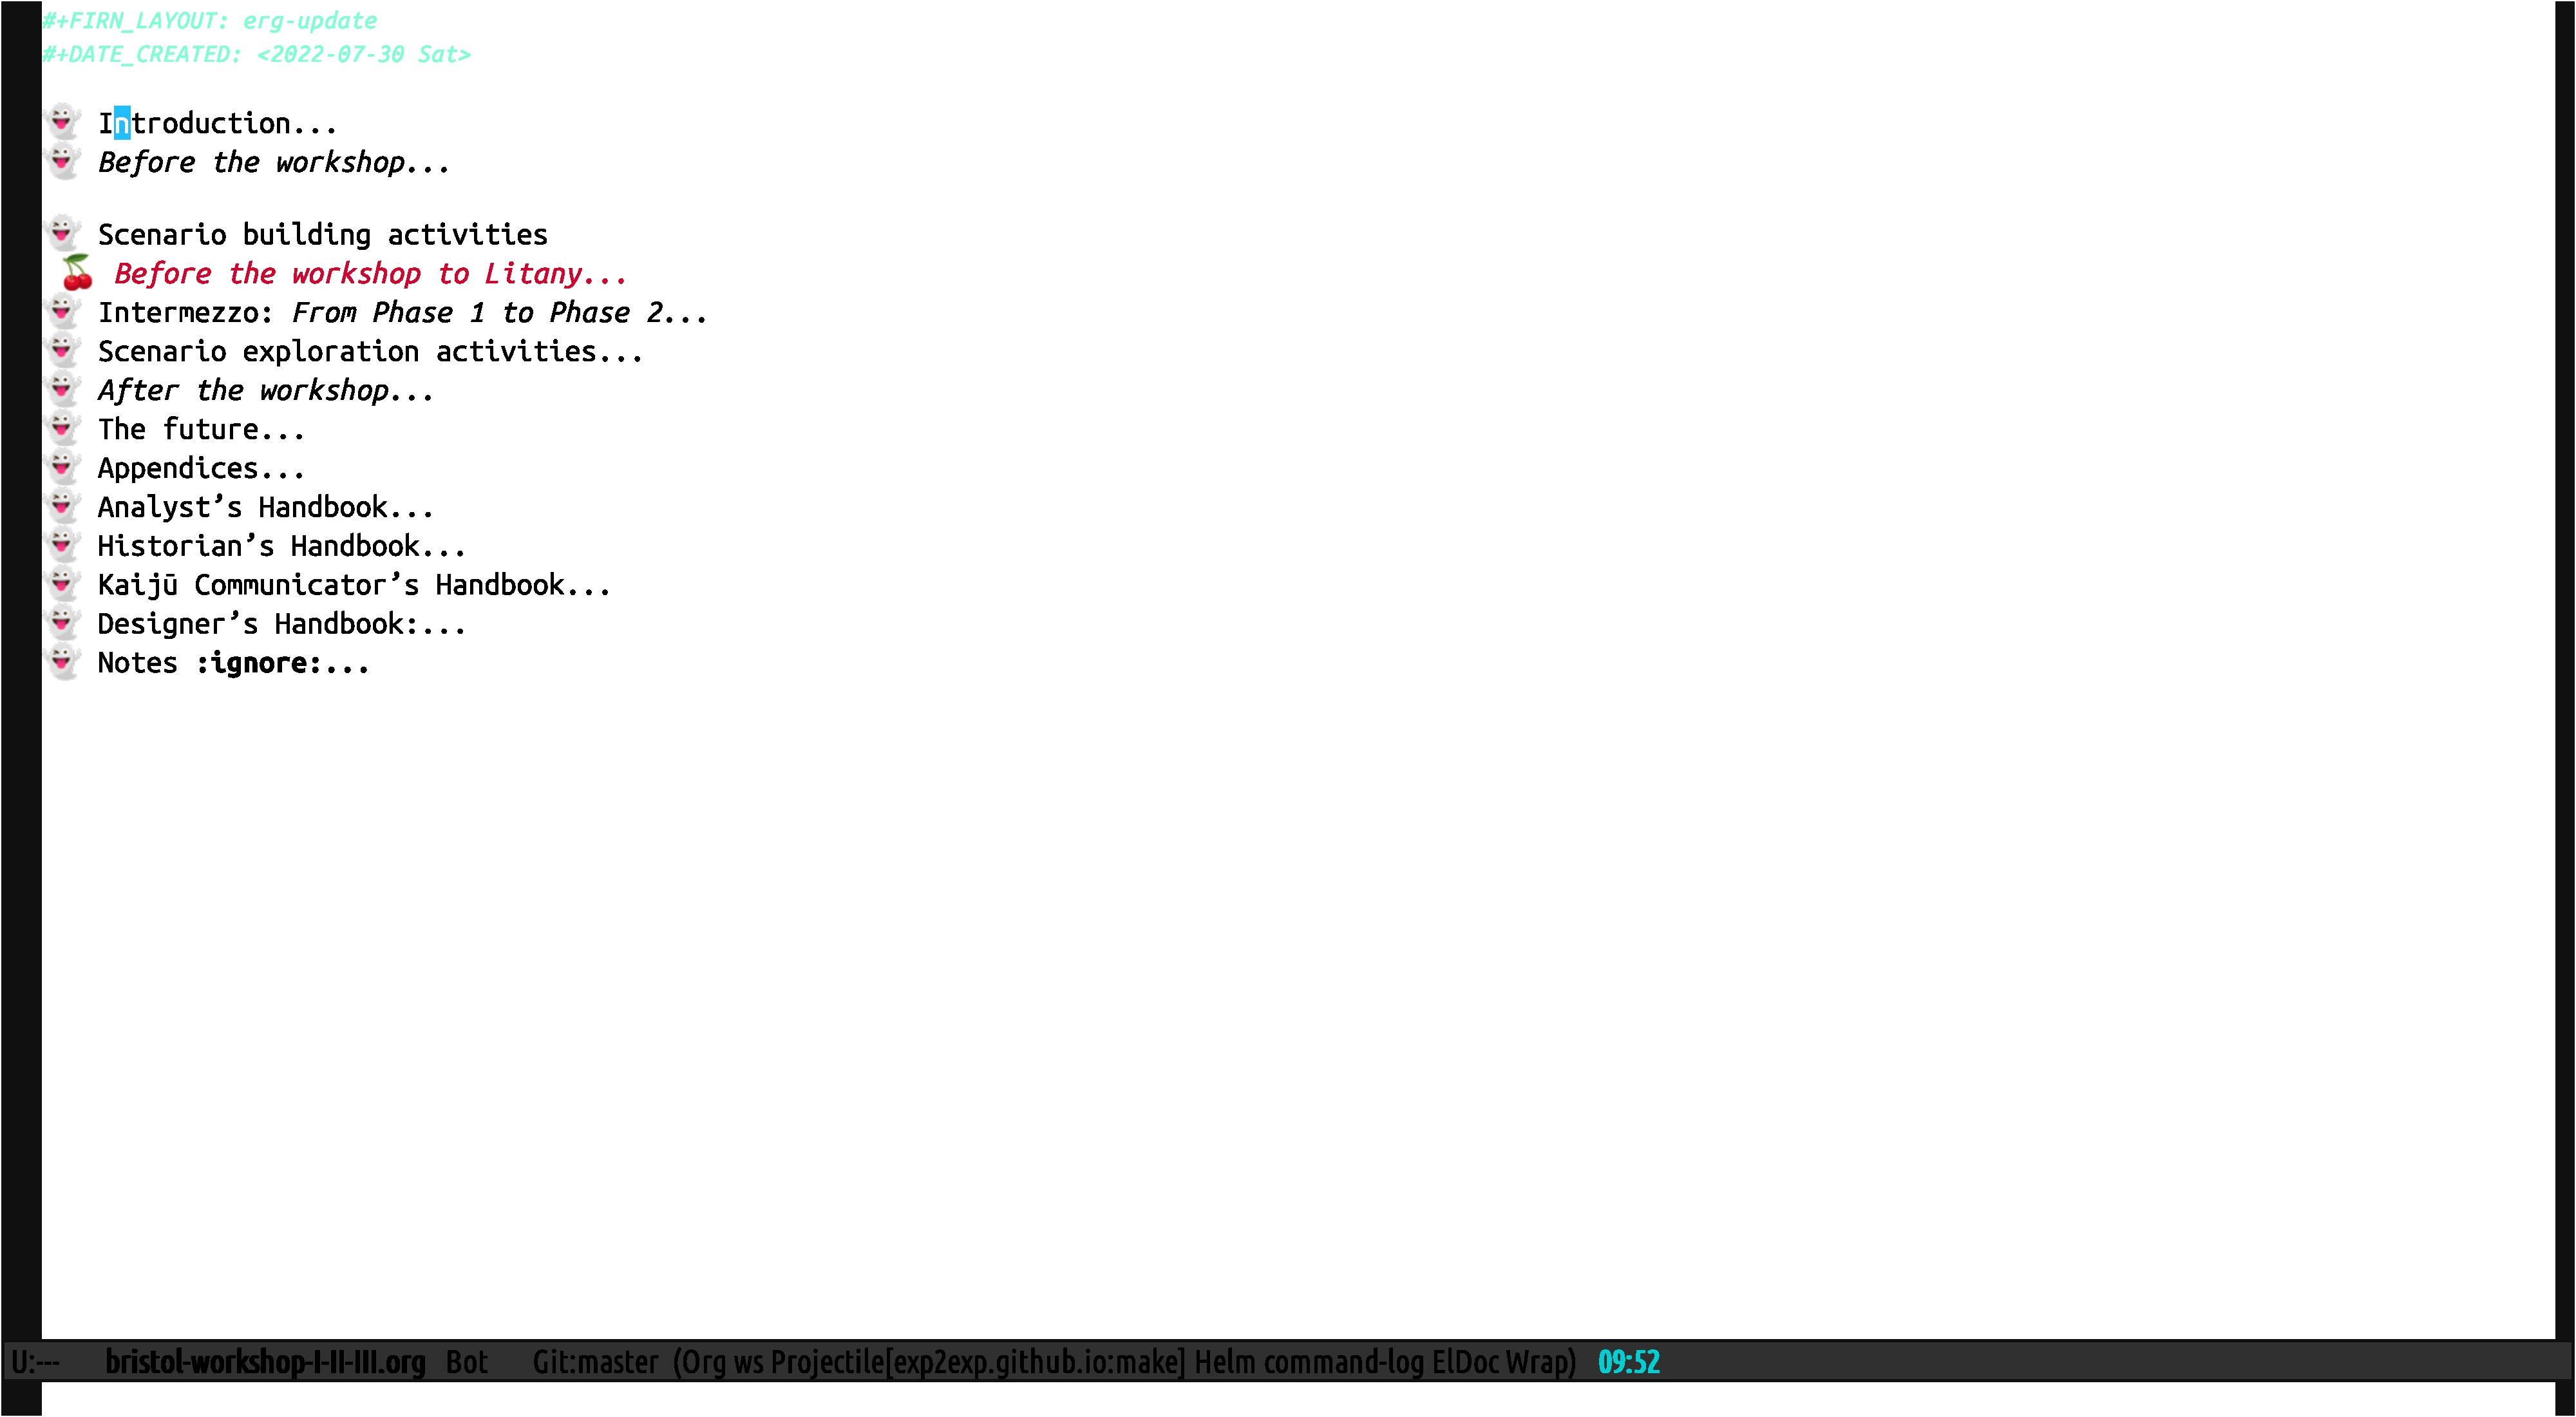
\includegraphics[clip, trim=1.1cm 18cm 45cm 2.5cm,width=.5\textwidth]{emacs.pdf}
\caption{\label{workshop-itinerary}}
\end{figure}

With that basic workflow in place, we refined the description of
constituent and adjacent activities using Design Patterns Language
methods.  We made a point of ensuring that the patterns we were using
had the opportunity to grow and evolve, and that their use fostered
the emergence of additional patterns.  We endeavour to show this
process within the paper.  As such, the paper includes a combination
of patterns that follow a formal template, and proto-patterns with
less structure.  We also made use of alternative (and intuitive)
pattern template structures as appropriate.  Proto-patterns without
any substructure are distinguished by a “💎” marker, evoking the
concept of \emph{pattern mining}.  In our view, additional formality
does not always help with communication, and we endeavour to show how
and when it is helpful, and when it is not.  For one thing,
proto-patterns admit multiple different formalisations, which offers
flexibility.  The downside is that their lack of explicit detail can
make them less replicable in other ways.  Throughout this work, design
patterns play the role of lightweight \emph{hypotheses}, structuring
the experience and receiving a degree of validatation or invalidation
through the workshop interactions.  Their survival to the next
workshop (or not) gives a sense of the evolutionary character of the
method.

On that note, we carefully reviewed the lessons learned after each
workshop, by using the Project Action Review template, or through less
formal but nevertheless detailed post mortems, and by looking for new
patterns.  Writing this paper is an opportunity for review at a deeper
rhythm.

\clearpage

\section{Case Study 1: “Going Meta” workshop at Anticipation 2022}

This workshop functioned as a more developed pilot of methods that we
already shared in earlier pilots (at PLoP 2021, at Oxford Brookes
Creative Industries Festival, and previously in more nascent forms).
Our aims were both to introduce the methods to attendees, and to
‘workshop’ the methods.  Our pitch was that we would help attendees to
establish a position of maximum leverage, exercising our “Critical
Anticipatory Capacities” using “Creativity, Innovation and New Media”
(two of the conference’s themes) to explore the future of
anticipation.

\subsection{Input patterns} \label{case1-inputs}

\emph{A small selection of patterns describing the workshop
activities, based on the more informal descriptions in our playbook,
were shared with workshop attendees in the form of “pattern cards”,
with which we transparently structured the workshop activities.  A
selection of these are shown in Figure \ref{cards}.  Several of these
are detailed below, along a few more-abstract patterns that
characterise the process.}

\begin{figure}
  \includegraphics[width=.9\textwidth,page=3,]{4-patternsa.pdf}
\caption{\label{cards}}
\end{figure}

\subsection*{DÉRIVE COMIX{\hfill (s)}}

\textbf{Context} you want to develop some future scenarios to explore with a group.\newline
\textbf{If} you have an group BUT everyone has their own experiences;\newline
\textbf{Then} Gather data.  For example: go for a walk \cite{debord},  or just look out the window wherever you are.  (Alternatively, close your eyes and conduct a mental exploration of your selected theme: what do you see in “your mind’s eye?”) Document what you see.  Follow up by preparing your materials to share in a succinct fashion, e.g., as photos, a screenshot, slides, sketches, a zine, a map, or some PostIt\textsuperscript{\textregistered} notes.

\smallskip
\noindent \emph{By itself, looking to the immediate surroundings only
gives an imperfect picture of how to develop a future scenario.
Direct observations might include little to no evidence of, say,
top-level government policy which likely is a major factor in the
future.  Two further patterns access more levels of meaning.}

\subsection*{MEANING MAP {\hfill (c)$\rightarrow$(m)$\rightarrow$(s)}}

\textbf{Context} We have collected images describing people’s worlds
(see {\sc Dérive Comics}).\newline \textbf{If} you want to distill
shared meaning BUT everyone has their own experience;\newline
\textbf{Then} talk together about the problems and opportunities that
everyone sees.  Maybe some of these will cluster together, or maybe
everyone will have their own different perspective: that’s OK.  You
can use these different viewpoints to get everyone on the same
page.\newline\smallskip

\subsection*{REINFUSE EXPERTISE {\hfill \cognitive}}

\textbf{Context} a group wants to build a {\sc Meaning Map}.\newline
\textbf{If} everyone has experience as a citizen BUT they also have
expertise;\newline \textbf{Then} begin by removing expertise to get
everyone on the same page, and subsequently reinfuse expertise to
enable richer and more complex thinking.\newline\smallskip

\subsection*{PATTERN LANGUAGE COMPONENTS {\hfill \sensory}}

\textbf{Context} In a collaborative setting with people who are new to
design patterns.\newline \textbf{If} new attendees are being invited
to create new patterns BUT the context, problem, solution language
brings assumptions that they may not be comfortable \newline \textbf{Then}
introduce more dynamic keywords such as HOWEVER (to describe a gap or
conflict), BECAUSE (to describe a set of operating causes), THEREFORE
(to describe a rationale based on related data) , and SPECIFICALLY (to
describe next steps) in order to help people talk about the different parts
of the patterns and build them up piece by piece.

\subsection*{FUNCTIONAL ROLES {\hfill \sensory}}

\textbf{Context} When building a new set of design patterns.\newline
\textbf{If} you have ideas about the components of a pattern BUT the
pattern hasn’t been fully formed yet.\newline \textbf{Then} introduce
some different perspectives to critique the pattern as it
develops.

\emph{In this workshop we tried aligning the {\sc Pattern Language
  Components} with {\sc Functional Roles}, as per “Phase II” in the
itinerary that follows.  In subsequent workshops, we decided to
separate these two dimensions more distinctly.}

\clearpage

\subsubsection{Workshop Itinerary}

\begin{mdframed}[backgroundcolor=blue!50,linecolor=blue!50]
  \noindent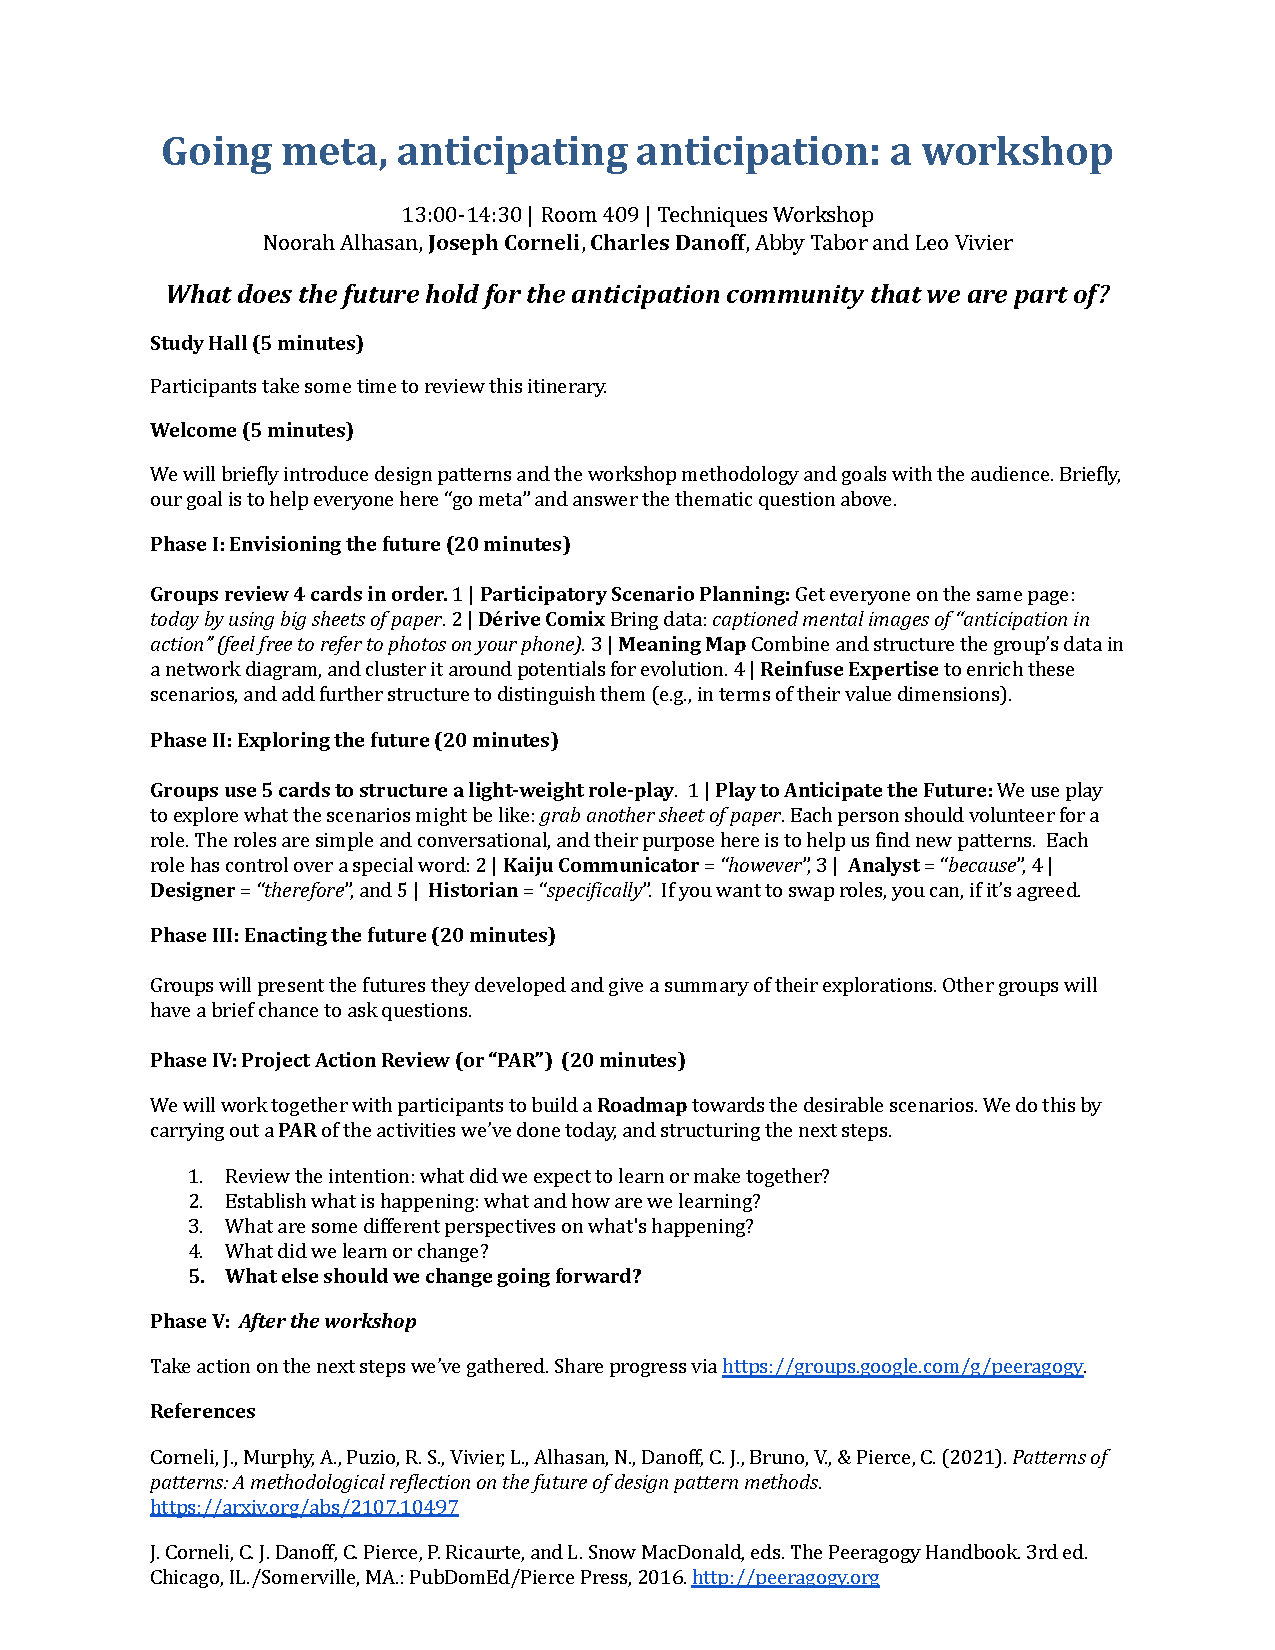
\includegraphics[width=\textwidth,trim={1cm 4.5cm 1cm 4.5cm},clip=true]{anticipation}
\end{mdframed}

\clearpage

\subsection{Output patterns}

\emph{The framing our workshop within the Anticipation conference suggested a pattern that could be repeated in other settings:}

\subsection*{GOING META{\hfill (c)}}\label{method1}
\label{sec:org958ff04}
\label{PLACARD}

\textbf{Context} In the course of working on a project
together.\newline \textbf{If} We may find a \textit{gap} between
our ideals and our methods;\newline \textbf{Then} Try “going
meta”, to explore how the project’s methods can be applied to
itself.\newline \textbf{Example} In a community that usually
focuses on anticipating the future for others, try inviting members of
the community to anticipate the future of the community.

\medskip

\noindent \emph{Reflecting on the attendees’ contributions, both in
terms of their concrete comments about the Anticipation community as
well as the way they interacted within the workshop gave rise to the
following proto-pattern:}

\subsection*{💎 INCREASE PARTICIPANT CONTROL {\hfill \motor}}

When organising a collaborative activity, participants should not
remain only a audience, or only deliver scripted lines.  Give them
increasing responsibility.

\clearpage

\section{Case Study 2: Public Space for Public Health}

This workshop was commissioned by Abby Tabor as part of her project
“Designing urban environments for human health: from the microbiome to
the metropolis”.  The aim was to gather attendees with an interest in
the project themes and work together to envision next
steps. Elaborations of these were developed by participants, and were
organised by facilitators using a software tool based on Org Roam and
Org Roam UI.
% \footnote{Demo: \url{https://hyperreal.enterprises/bristol}}

\subsection{Input patterns}

Alongside the main components of the initial workshop, we looked for
new methods to {\sc Increase Participant Control}.  In particular, we
generated some further articulations of the {\sc Functional Roles} to
help with this.

The patterns are presented here with a mnemonic symbol based on the
chess set; at the workshop, participants were provided with physical
manipulatives from a chess set that helped them get a grasp on the
roles, along with new pattern cards with the text on.

\subsection*{TIME TRAVELLER {\chess ♕} {\hfill \sensory}}

\textbf{Question} \emph{What has happened in the past, what could
happen in the future?}\newline
\textbf{Role} To provide historical context and
anticipate alternate futures.

\subsection*{WRINKLER {\chess ♘} {\hfill \motor}}

\textbf{Question} \emph{What could go wrong? }\newline
\textbf{Role.} Consider what might derail or counter
the proposed solution.  Each wrinkle can be assigned a level of
perturbation (from low to high).

%\textbf{Example} Everyday roadmap languages include both iconic map and road sign symbols; when people are confused or lost they may ask for help or try to find their own way back to the road using other informal languages.
\subsection*{ANALYST {\chess ♗♝} {\hfill \cognitive}}

\textbf{Question} \emph{What are the moving parts?}\newline
\textbf{Role 1} Consider the current challenge and all the components
of the potential solution (actors, resources, institutions). Identify
and orchestrate the dynamic network of these components.\newline
\textbf{Role 2} Consider the other challenges specified beyond the
current focus.  Identify and orchestrate the integration of these
components relevant to the present challenge.

\smallskip

\noindent \emph{(We also characterised some roles which would be
filled by offsite and onsite facilitators.)}

\subsection*{FACILITATOR ROLES {\hfill \cognitive}}
\textbf{Context} Developing a collection of interrelated design
patterns.\newline \textbf{If} you are getting ideas from participants
who play {\sc Functional Roles} BUT the ideas aren’t all connected
with each other in a structured way.\newline
\textbf{Then} introduce
facilitator roles to help structure the collection.\newline
\textbf{Specifically}, {\sc Linkers}, and {\sc Reflectors} are two
roles that we have found useful.

\subsection*{LINKERS {\chess ♖}{\hfill \sensory}}

\textbf{Question}
\emph{How do proposed scenarios build into patterns across layers, and how do they interact within the constellation?}\newline
\textbf{Role.} Data wrangling as it comes in, providing visualisation of patterns and interconnections.

\subsection*{REFLECTORS {\chess ♔}{\hfill \cognitive}}

\textbf{Question} \emph{How is the scenario evolving?}\newline
\textbf{Role} To appraise each scenario, provide a format for reflection (PAR), make decision to continue, reset, end.

\subsection{Itinerary}

\begin{mdframed}[backgroundcolor=blue!50,linecolor=blue!50]
  \noindent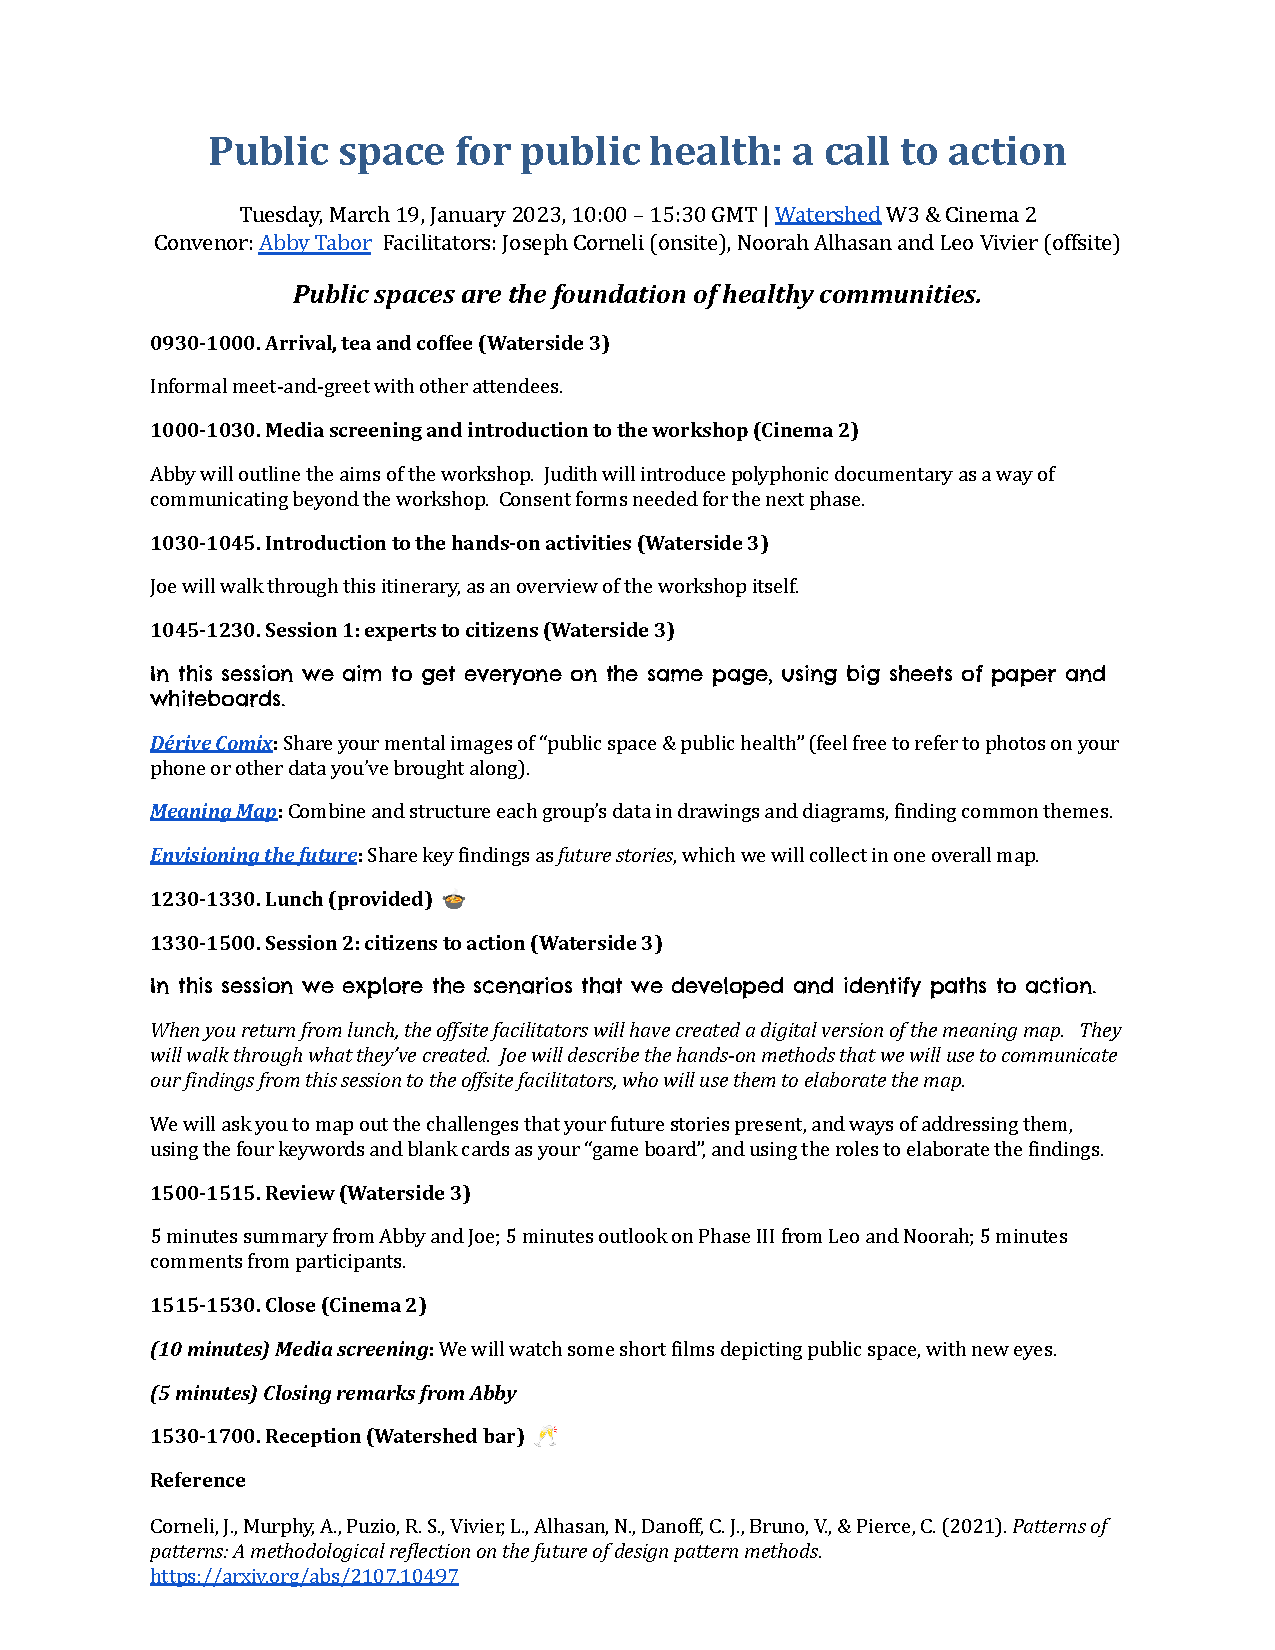
\includegraphics[width=\textwidth,trim={1cm 3.2cm 1cm 4.5cm},clip=true]{bristol}
\end{mdframed}

\subsection{Intermediate artefacts}

Intermediate artefacts generated within the workshop included mindmaps
created with participants, on paper.  We used a graphical template
following the outline of the Causal Layered Analysis layers to explain
the workshop’s overall workflow, and also asked participants to use a
version of this diagram as a “grid” for note-taking within Phase I, to
encourage them to work from their observations to the core underlying
themes and issues.  Participants then clarified these core themes in a
share-back process, and in Phase II, developed them further in the
form of shared future stories, outlining paths to action.  Photos in
Figure \ref{ExampleParticipantPattern} show the movement from initial
sketching at the litany level within small groups, to a collection of
themes shared across groups, to Phase II work using {\sc Pattern
  Language Components} to identify both general and specific
possibilities for action.

\begin{figure}
  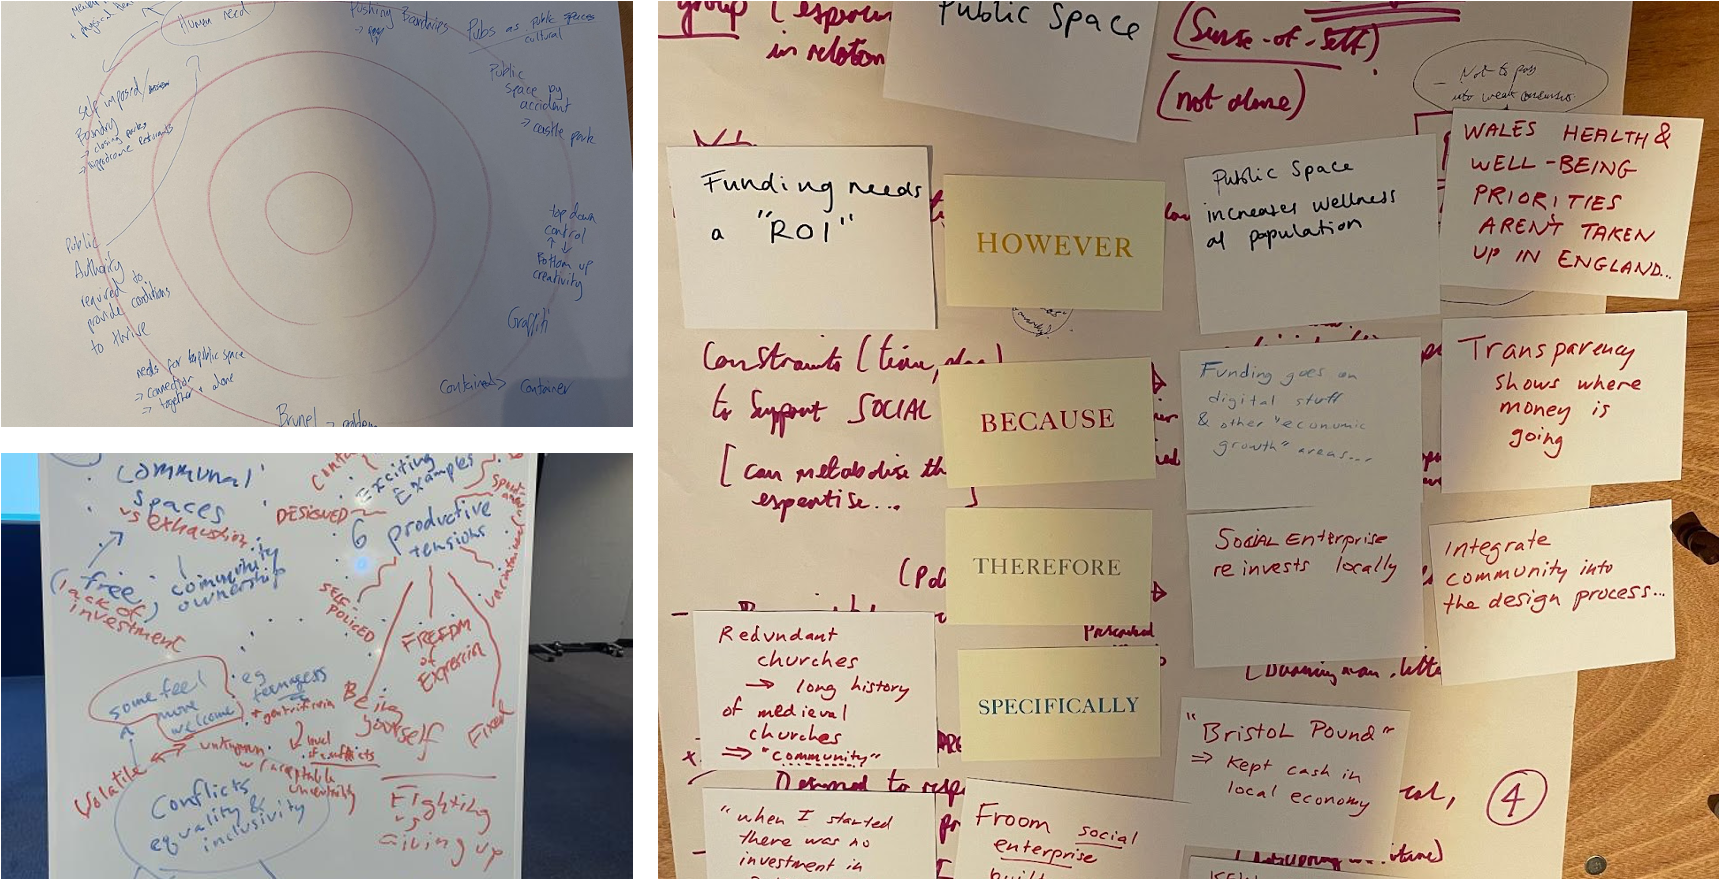
\includegraphics[width=\textwidth]{PatternProcess.png}
  \caption{\label{ExampleParticipantPattern}}
\end{figure}

\clearpage 

\subsection{Output patterns} ~
\smallskip

\noindent \emph{Reflecting on the contributions of the workshop
convenor and special guest, we observed a pattern that could be used
in subsequent workshops.}

\subsection*{CONTEXT SETTING {\hfill \cognitive}}
\textbf{Context} A workshop or other working context has been
convened.\newline \textbf{If} the facilitators have ideas that they
would like to explore with attendees BUT these ideas are not top of
mind for attendees.\newline \textbf{Then} do some context-setting,
e.g., showing videos, giving a short talk about why people have been
invited and describe the hoped-for outcomes.

\smallskip

\noindent \emph{Participants created several patterns by making use of
the {\sc Pattern Language Components} and {\sc Functional Roles}.
They presented below in summary proto-pattern form.  These summaries
condense details which developed in the workshop using manipulatives
(cards and chess pieces) with greater articulation, but less
coherence.}

\subsection*{💎 CONTESTED SPACE{\hfill \sensory}}\label{pat:contested-space}

So-called public space doesn’t always feel welcoming to all members of the public.  It can be overrun with antisocial behaviour.  It can feel exclusionary, or uninviting.  It can be the site of conflict. However, the need for complex uses of public space does not mean that each space needs to support every use equally.

\subsection*{💎 REBALANCE SOCIAL SERVICES{\hfill \motor}}\label{pat:rebalance-social-services}

Welfare-related services should be supplied in balance with local needs, though they often are not. Can varied expertise be integrated in a similar way to the domain-specific skills practised by Médicins Sans Frontièrs to address complex local challenges?

\subsection*{💎 FUNDING OF PUBLIC SPACE{\hfill \cognitive}}\label{pat:funding-of-public-space}

Even though public space is known to increase wellness in the population, well-being priorities that would lead to increased funding for public space aren’t universally adopted.  In order to make the benefits of such investment clear, increase transparency around investments in public welfare, e.g., create register of impacts of local social enterprises.

\medskip

\noindent \emph{(The right-hand panel of Figure
\ref{ExampleParticipantPattern} shows how participants elaborated the
    {\sc Funding of Public Space} proto-pattern on the day, using the
    {\sc Pattern Language Components} that we provided as keywords on
    index cards; the others listed above were diagrammed out similarly
    on the day.)}

\medskip

\clearpage
\section{Case Study 3: Open Research Futures}

This workshop was developed as an “Away Day” for faculty and staff
members at Oxford Brookes University.  The aim of the workshop is to
elaborate the institution’s open research strategy relative to its
existing organisational strategy.  Methodologically, this workshop
builds on a pre-seeded Org Roam network of interlinked themes and an
additional activity that enlists attendees in taking concrete actions
on the identified next steps.  This itinerary reused the language
“experts to citizens”, “citizens to action” from the previous workshop
(with a slight variation suited to the context).  These phases mirrors
the {\sc Dérive Comix}—{\sc Meaning Map}—{\sc Reinfuse Expertise}
structure introduced earlier.

\subsection{Input Patterns}

\subsection*{DO YOUR RESEARCH{\hfill\sensory}}
\textbf{Context} Prior to beginning a formal workshop or other participatory research activity.\newline
\textbf{If} it looks like it will be possible to do participatory research BUT the participants haven’t begun speaking with each other yet.\newline \textbf{Then}
start doing the research in a more centralised way before inviting direct collaboration, in order to give participants something to engage with.\newline
\textbf{Example} In the current setting, this pre-research included 1-to-1 interviews with about half of the invitees, as well as internet research to find and explore related scenarios developed by others.\footnote{\url{https://royalsociety.org/topics-policy/projects/research-culture/changing-expectations/visions-of-2035/visions-of-2035-materials/}}

\subsection*{STRUCTURE CONVERSATIONS{\hfill\cognitive}}
\textbf{Context} Having convened a workshop or other participatory research activity.\newline
\textbf{If} unstructured discussions are likely to take lots of time but without yielding concrete benefits.\newline \textbf{Then}
structure the discussions around shared interests to move things forward more effectively.\newline
\textbf{Example} At this workshop, we decided to group participants around tables according to the faculty where they were employed (or most closely alignd, in the case of university-level support staff).

\subsection*{THE FUTURE BEGINS NOW{\hfill\motor}}
\textbf{Context} Having developed possible next steps.\newline
\textbf{If} appears that leaving without concrete commitments means
concrete actions are less likely to take place.\newline \textbf{Then}
introduce early actions within the
collaborative setting to create commitment.\newline
\textbf{Example} One way to build commitment would be to ask people to develop and share a method for a small-scale experiment that they plan to carry out.

\clearpage

\subsection{Itinerary}

\begin{mdframed}[backgroundcolor=blue!50,linecolor=blue!50]
  \noindent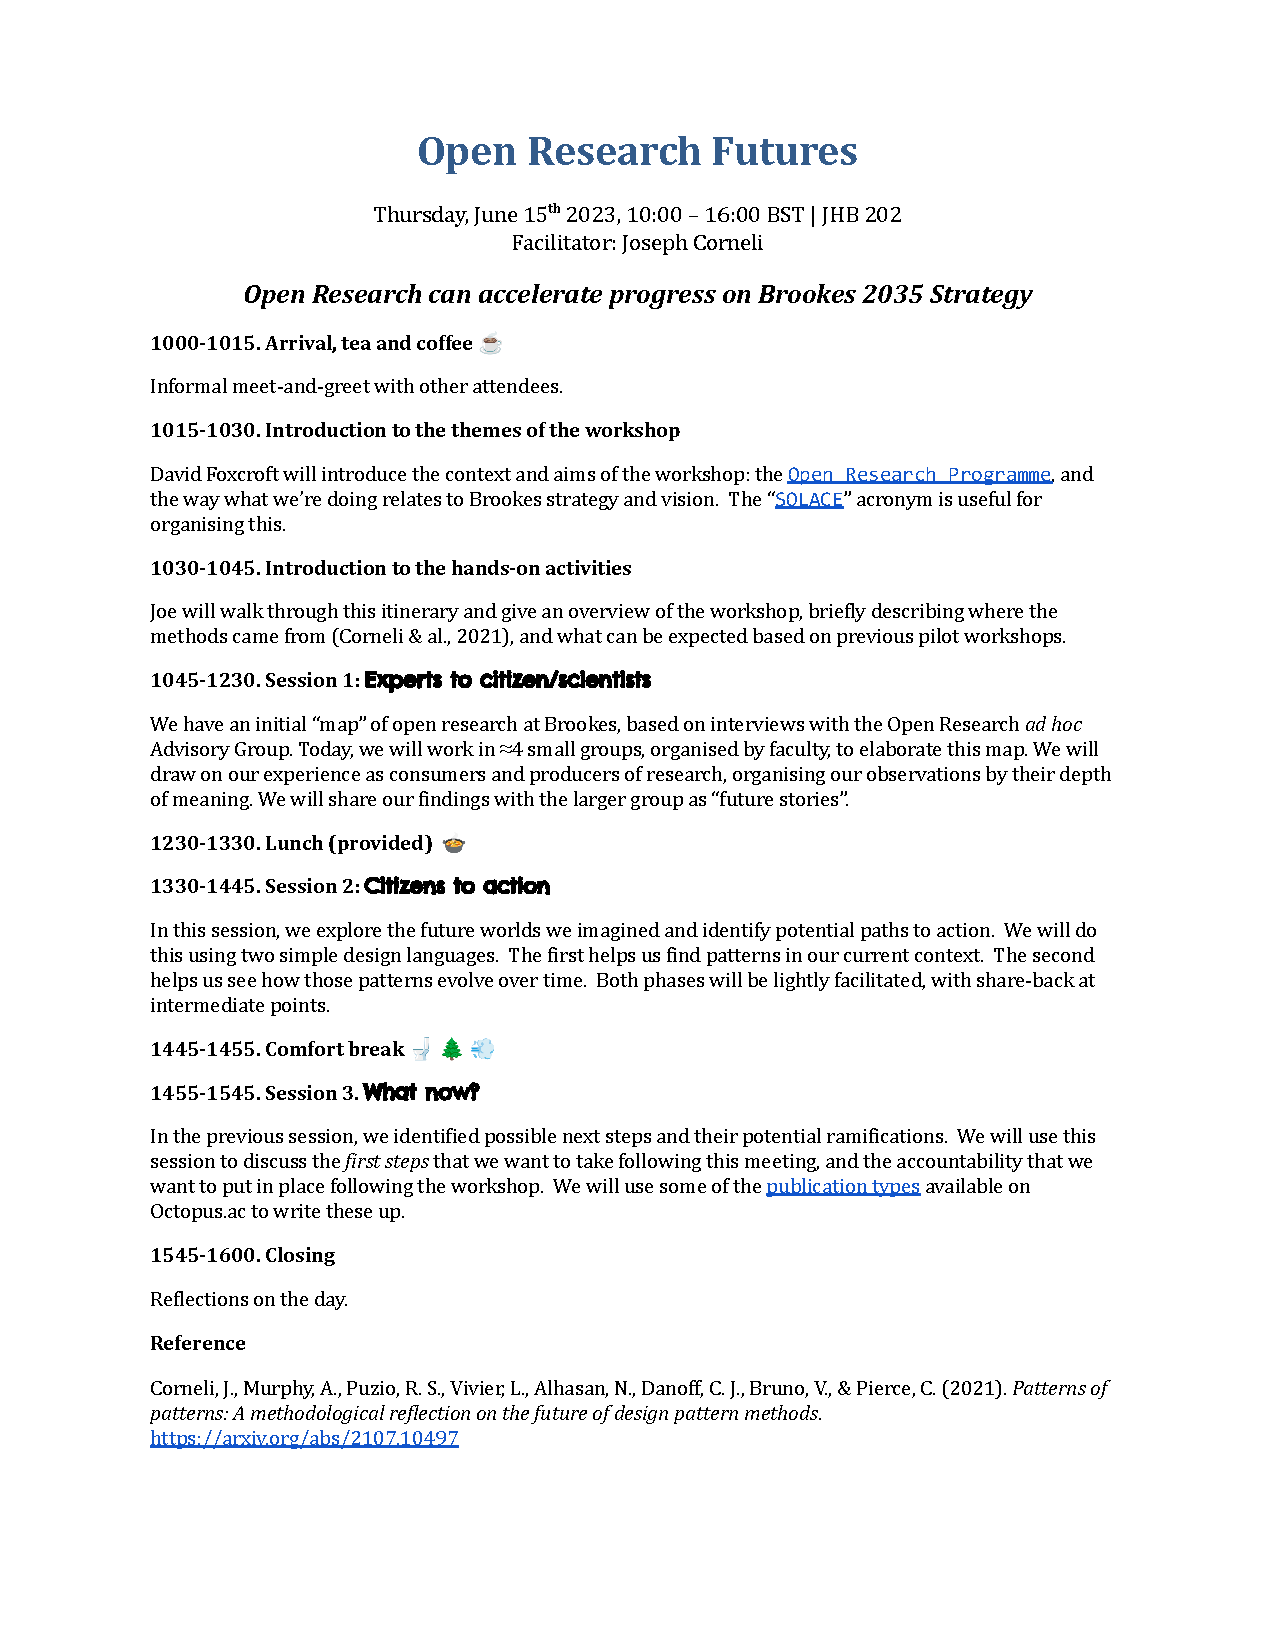
\includegraphics[width=\textwidth,trim={1cm 5.5cm 1cm 4.5cm},clip=true]{brookes}
\end{mdframed}

\clearpage

\subsection{Output Patterns}

\begin{figure}
  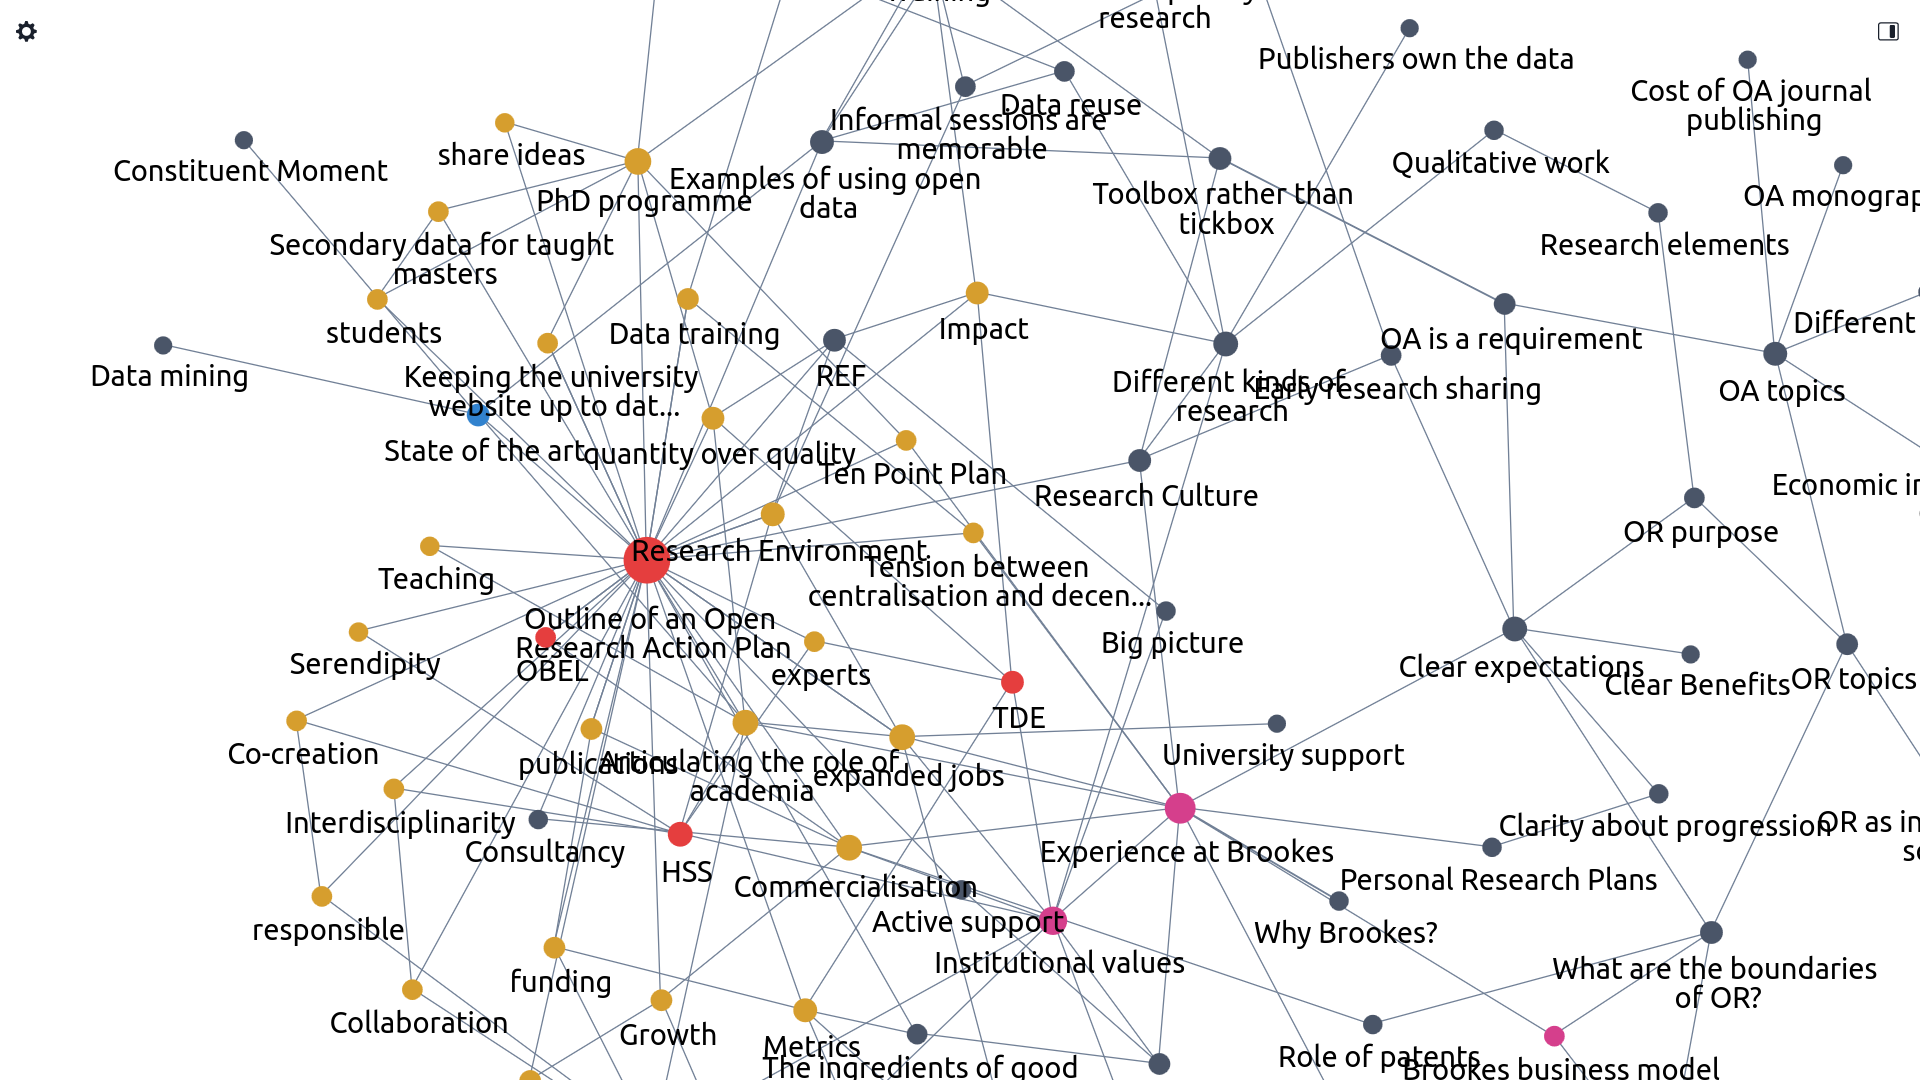
\includegraphics[width=\textwidth]{org-roam-screenshot.png}
  \caption{\label{Org-Roam-Screenshot}}
\end{figure}

\subsection*{💎 STRUCTURE OUTPUTS{\hfill\motor}}
Having gathered themes from a participatory project, they may have
some explicit (e.g., because of how the information was gathered,
cf. {\sc Structure Conversations}).  Additional structure can be
created, if you link intermediate artefacts into a relevant template.

\emph{In this setting, we used a template provided by the UK
Reproducibility Network for developing an Open Research Action Plan
\cite{orap-template} — itself a complex pattern.  We linked the themes
discussed in the workshop into this template, to form a bullet-point
draft of an action plan, incorporating the next steps and concerns
raised by attendees.  We did not specifically include all of the
background that appeared in our earlier interview (cf. {\sc Do Your
  Research}).  Figure \ref{Org-Roam-Screenshot} shows all of this
material in an intermediate form, where we used Org Roam to analyse
the workshop themes (per the {\sc Linkers} pattern, above).}



%% \subsection*{PLACARD: A Synthesis of PAR, CLA, and DPL}
%% \label{sec:orgd924cd6}
%% \label{methods_summary} We are now in a position to explain how PAR, CLA,
%% and DPL combine into one holistic pattern, in Leitner’s sense of a
%% complete methodic description \cite{leitner2015a}.  We will write this
%% down using the classic DPL format: describing the associated
%% \emph{context}, the \emph{problem} denoting a conflict, together with a \emph{solution}.
%% As it happens, the three acronyms introduced earlier can be combined and remixed
%% to provide a title for this pattern.
%% $$\textrm{PAR}+\textrm{CLA}+\textrm{DPL}=\textrm{PLACARD}$$
%% This accurately suggests that
%% the methods need not be run in a fixed order, but are interwoven together.
%% %\paragraph{PLACARD}
%% \label{sec:org958ff04}
%% \label{PLACARD}

%% \begin{itemize}
%% \item \textbf{Context}: In the course of working on a project: \emph{we use the PAR to get a sense of our working context}.
%% \item \textbf{Problem}: Although we may encounter many difficulties in this context, our effort to understand them faces a central \textbf{challenge}, namely the fact that the problems span different layers and scales of complexity, so it can be hard to understand where the difficulties actually come from: accordingly, \emph{we use the CLA to understand and frame the problems and their interconnections}.
%% \item \textbf{Solution}: Once we have grasped the problem, we need to elaborate an actionable solution that remains adaptable to ongoing changes in the context: \emph{we use DPL to elaborate the solution (returning to PAR and CLA as needed)}.
%% \end{itemize}


\section{Case Study 4: CIS 9590, Information Systems Development Project}

\subsection{Introduction the course from the instructor, Mary Tedeschi}
% Mary please write in this file

CIS 9590 is Information Technology Project Design and Management is the  ``Computer Information Systems'' (CIS) capstone project course for the CIS major wherein the students will apply concepts and techniques from prior course work, to design, develop, and create an implementable application for a working information system of an actual business. It also focuses on the design and management of systems to meet the increased need for information within an enterprise. The course exposes students to the fundamentals of IT project management required for the successful implementation of IT-based systems. The course presents tools and technologies for project definition, work breakdown, estimating, planning and scheduling resources as well as monitoring and control of project execution. Students utilize knowledge gained from prior coursework, and work in groups to design and manage an Information Technology project.  During my first semester, Spring 2020, teaching with the students using whatever development tools they were familiar with, I noticed this to be a problem so with this knowledge I changed the course to require the use of Intel One API.  This did not get implemented until Fall 2021.  I actually taught the course three times before requiring students to use the same software tool uniformly.  The course was a 3 hour course, first face-to-face.  Then synchronous online only.  In Fall 2021 we changed to 75 minutes in person and online (hybrid).  Students had to self-teach Intel One API with the use of tutorials and a buddy system.  The students seemed to have the necessary skills to learn enough of the software to create an implementable application.  This semester, Spring 2023, the students really seemed to lack the coding skills.


\subsection{Our use of “Patterns of Patterns” within the course}
\label{pop1-in-cis9590}
We used the paper “Patterns of Patterns” as a focal text with three
successive cohorts of CIS 9590 students.  The course syllabus is
focused on developing group projects with a computer programming
component.  Our hope was that the topics in the paper would inspire
them with new ideas about design and collaboration.  We focus
primarily on the latest iteration of the course (Spring 2023), in
which we made the most explicit use of the methods described above.
Figure \ref{cis-9590-anticipations} shows some of our anticipations of
the relevant concerns that apply in this context.

\begin{figure}[h]
  \begin{tabular}{cc}
    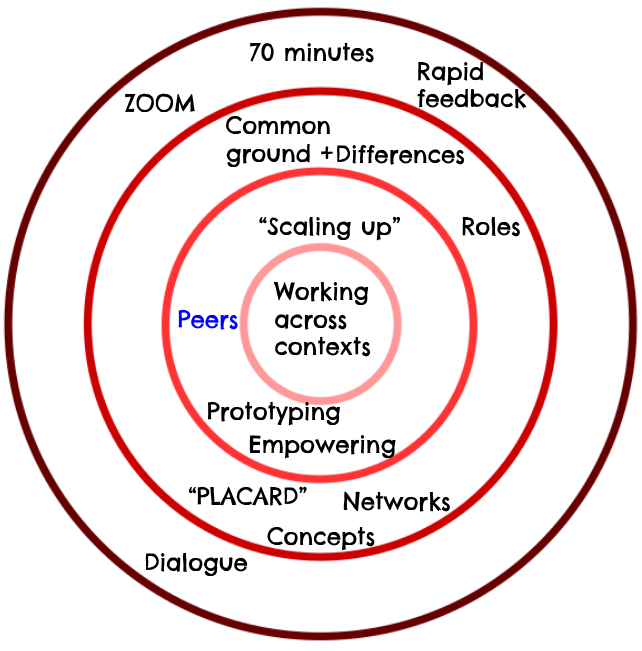
\includegraphics[width=.45\textwidth]{UsCLA.png} &
    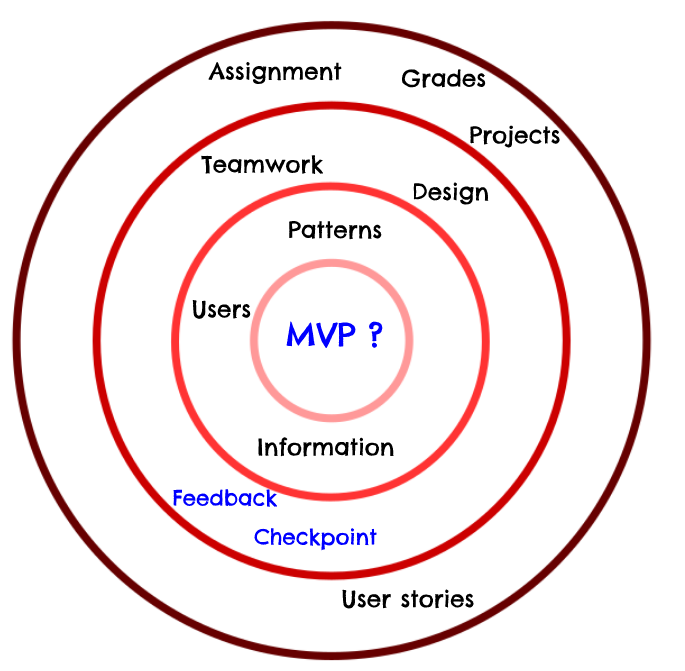
\includegraphics[width=.45\textwidth]{ThemCLA.png}
  \end{tabular}
\caption{Diagrams inspired by Causal Layered Analysis describing our working context as guests in CIS 9590 (left), and our initial understanding of the students’ working context (right).\label{cis-9590-anticipations}}
\end{figure}

Each year, students asked many thoughtful \emph{questions} about the
paper; they also produced their own \emph{written response} to the
paper, engaging the original paper in depth; and in the latest run, we
offered some in-class \emph{exercises} based on the workshop methods
described above.  Reading these written responses showed that the
students had not only understood the main ideas of our paper, but
added to them.  In effect, they created alternative imaginaries for
the paper’s history and future.  For instance, in their 2022 ‘case
study’, they generated a “Recommendation and Implementation Plan”
which proposed specific actions which a group could take based on our
ideas; and, in 2023, the students produced a slide presentation based
upon our paper, exploring its relationship to themes such as “emerging
technology”.

Building in part on these student responses, we will now present our
reflections using the Causal Layered Analysis layers.

\subsubsection{Litany}
Initially our paper was introduced as a contemporary reading, relevant
to the “CIS” theme.  Mary chose a contemporary paper in part because
students would not be able to “cheat” in their reports, because our
paper wasn’t described extensively on Sparknotes or similar.  Along
with this (intentional) challenge, CIS 9590 students encountered a
range of more or less predictable problems, e.g., many felt a lack of
confidence with coding.  The students came to the course with a
variety of different backgrounds (e.g., Python vs C++) which
contributed to some friction with this course.

\subsubsection{System}
Whereas in our rounds of earlier participation we were more there for
enrichment, in the most recent iteration our contributions were more
closely integrated into the main activities of the course. We attended
more sessions, including one in which we attempted to run a short
version of the workshop with attendees.  This allowed us opportunity
to interact with the students on an ongoing basis as they designed and
implemented theie projects.  Furthermore, Mary attended at least as
many meetings of the Peeragogy project, fostering an exchange of ideas
and viewponts between these two contexts. In the short term, this led
to productive synergy and, in the long term, could lead to our
pedagogical and peeragogical initiatives becoming more integrated into
a larger system. This collaboration continued post-semester, insofar
as Mary invited the students to express interest in possible
internships in the Peeragogy project.

\subsubsection{Worldview}
Students were thinking about their future careers.  What they wanted
to get out of the course (e.g., becoming a well-paid data scientist or
business leader) at times had some friction with the practical reality
of the course requirements, in which they had to deliver a concrete
hands-on working project, without being able to rely on employees.
PLACARD wouldn’t be of much direct help with the technical challenges
they faced, but we hoped it could help them organise their work in a
sensible way.  More informally, the ideas underlying PLACARD informed
our comments; for example, in a session with Mary in which we
‘workshopped’ CIS 9590 with other peeragogues, discussants suggested
adding more touchpoints for peer learning and feedback.

\subsubsection{Myth}
A deep metaphor within the classroom setting is \emph{pedagogy}.
However, the methods that we brought as guests was more linked with
our experience of \emph{peeragogy}.  In the new shared context, these
two perspectives begin to integrate.  Mary as a host exercised the
value of \emph{xenia} by bringing us into her course as guests.  The
possibility of student internships within the Peeragogy project would
create the reciprocal opportunity for further student practice with
CIS skills in an applied context, helping to build tools and platforms
for peer learning and peer production (including through use of
pattern methods).  Indeed, the particular combination of peer learning
and formal education developed here led us to wonder how far off the
Peeragogy project might be from being able to support informal
learning of relevant programming concepts (preliminaries to CIS 9590)
or applied computing projects (an analogue of CIS 9590).

\subsection{Proto-patterns describing the experience, by a CIS 9590 student, Manvinder Singh}\label{sec:manny-protopatterns}

%% Introduction:
%% During my final project class led by Professor Mary Tedeschi, the research paper 'Pattern of Patterns' and its authors played a pivotal role in shaping my project decisions. The authors' active engagement in our Zoom sessions provided invaluable insights into project layout, helped me avoid common mistakes, and encouraged a scalable and adaptable approach. Their active engagement and promises to come again in the following weeks to see progress on everyone’s individual project kept the butterflies, nervousness, and willingness to deliver all alive at the same time.

\subsection*{💎 ENGAGEMENT AND GUIDANCE{\hfill \motor}}
The authors of ‘Pattern of Patterns‘ actively participated in our
class, to share expertise and create a collaborative learning
environment. Their presence allowed us to gain deeper insights into
the paper's concepts and methodologies, leading to innovative project
approaches. By closely studying the patterns of patterns identified in
their research, I gained a fresh perspective on project organization
and established a logical and coherent structure.

\subsection*{💎 AVOIDING MISTAKES{\hfill \cognitive}}
The authors' insights helped me navigate common project development
pitfalls.  Through their emphasis on effective documentation, regular
testing, and thorough project planning, I was able to avoid costly
errors.  Their guidance ensured a consistent progress trajectory and
maintained the professionalism of my final project.

\subsection*{💎 SCALING AND ADAPTABILITY{\hfill \cognitive}}
‘Pattern of Patterns’ underscored the importance of scalability and
adaptability in project design.  By considering future technologies
and incorporating modular elements, I aim to seamlessly adopt new
advancements.  In particular, I focused on building a flexible
framework that could easily accommodate emerging technologies.

\subsection{Further reflections}

Our anticipations (Figure \ref{cis-9590-anticipations}) didn’t
precisely match our reflections at the end of the course.  The missing
steps on the way to the eventual synthesis could suggest further
patterns, including elaborations on Manvinder Singh’s proto-patterns
that give more specificity.

%% Conclusion:
%% The research paper 'Pattern of Patterns' and its authors significantly influenced my final project experience. Their engagement, guidance in project layout, avoidance of common mistakes, and focus on scalability and adaptability empowered me to make informed decisions. By observing patterns and applying their insights, I successfully developed a project that thrived in the dynamic landscape of technology. I am grateful for the authors' contributions, which shaped my final project journey under Professor Mary Tedeschi's guidance.

\section{Discussion}

We presented the patterns that we developed and used over successive
runns of our workshop, in approximately chronological order, aiming to
show how the use of certain patterns help to give rise to the
``seeds'' of new patterns.  The evolving workshop method is a pattern
language which operationalises the PLACARD pattern.

The first workshop mixed {\sc Pattern Language Components} with {\sc
  Functional Roles}, putting participants in the thick of a
pattern-related dialogue.  While this led to interesting
conversations, it was more work to extract any patterns.  We did find some useful process
patterns this way, such as {\sc Increase Participant Control}.  We employed what we learned in subsequent
runs.   Within the second workshop, a more distinct use
of the {\sc Pattern Language Components} helped the participants come
up with their own patterns.

There is an interesting interplay between content-level patterns like
these, and process-level patterns.  For instance, the workshop is akin
to a public space; further development of the associated tools might
make it even more of a public resource — somewhat like Wikipedia, but endorsing the contribution of original research, not forbidding it.  Already, the workshop is a context in which to do a kind of rapid, local, open research.

In order for any pattern-informed research to work well, we should be gathering evidence for or against the salience of the patterns that are elaborated.  The Octopus platform mentioned in the itinerary for Case Study 3 uses several data types that follow the rough outline of a scientific paper, \emph{viz.},
Research Problem,
Rationale/Hypothesis,
Method,
Results,
Analysis,
Interpretation,
Real World Application, and
Peer Review.
The formulation of an Octopus-like platform for recording and reporting on design patterns would probably need to change somewhat — but the \textbf{Problem}, \textbf{Rationale}, \textbf{Method}, and \textbf{Results} components are reasonably familiar for pattern authors.

Table \ref{summary} summarises the patterns that were described in
this paper, pulling them together from across the separate cases studies.  The table shows the patterns grouped in a way that elaborates
our use of “PAR”, “CLA”, and “DPL” methods (summarised in Section \ref{sec:org7c32ecc}) with a more rounded
description of the purposes that these methods serve.  Further work
would be needed to fully describe the patterns’
application domains, with evidence of the kinds of results that can be expected, and to describe their interconnections as a pattern language.

\begin{table}
  \begin{tabular}{rll}
Sensory: &\\
&  {\sc Contested Space}& ‘complex uses of public space’ \\
&  {\sc Dérive Comix}& ‘document what you see’ \\
&  {\sc Do Your Research}& ‘start doing the research in a more centralised way’\\
&  {\sc Functional Roles}& ‘introduce some
different perspectives’ \\
&  {\sc Linkers}& ‘providing visualisation of patterns and interconnections’ \\
&  {\sc Pattern Language Components }& ‘build them up piece by piece’\\
&  {\sc Time Traveller }& ‘provide historical context and
anticipate alternate futures’\\
%\hline
Cognitive: && \\
&{\sc Avoiding Mistakes}& ‘navigate common project development pitfalls’\\
&{\sc Context Setting}& ‘describe the hoped-for outcomes’\\
&{\sc Funding of Public Space}& ‘create a register of impacts’\\
&{\sc Facilitator Roles}& ‘structure the collection’\\
&{\sc Going Meta}& ‘explore how the project’s methods can be applied to
itself’\\
&{\sc Reflectors}& ‘appraise each scenario’\\
&{\sc Reinfuse Expertise }& ‘enable richer and more complex thinking’\\
&{\sc Structure Conversations}& ‘structure the discussions around shared interests’\\
&{\sc Scaling and Adaptability}& ‘aim to seamlessly adopt new advancements’\\
&{\sc Analyst }& ‘identify and orchestrate the dynamic network’ \\
%\hline
Motor: && \\
&{\sc Structure Outputs}& ‘link intermediate artefacts into a relevant template’\\
&{\sc Engagement and Guidance}& ‘create a
collaborative learning environment’\\
&{\sc Increase Participant Control}& ‘participants should not remain only an audience’\\
&{\sc Rebalance Social Services}& ‘address complex local challenges’\\
&{\sc The Future Begins Now}& ‘introduce early actions within the
collaborative setting’\\
&{\sc Wrinkler }& ‘what might derail or counter
the proposed solution’\\
%\hline
*\phantom{xxx} & \\
&  {\sc Meaning Map }& ‘get everyone on the same
page’\\
  \end{tabular}
  \smallskip
  \caption{“Patterns of Patterns” pattern catalogue\label{summary}}
\end{table}

\section{Conclusion}

We hoped that running these workshops would help us design the next
steps for our platform and process, and this seems to have been
successful.  As an immediate outcome, we developed the “PLACARD
workshop” — now retitled “Open Future Design” — across several
successive runs in different organisational contexts in a way that
makes it more robust.  This relative success notwithstanding, it is
worth recalling that our initial intention in Patterns of Patterns
\emph{was to support distributed collaboration across contexts}.

The informal pattern-based review of our evolving work, presented
here, is a good start.  Software development could carry this work
further.  A not-so-distant future for Org Roam would allow several
facilitators to make notes in near real-time into a shared map, and
with some more fine tuning of the Emacs interface, a similar workflow
could be used directly by workshop attendees, even across different
contexts.  Many rich dialogues might ensue — integrating concepts from
fields as disparate as future studies, health sciences, open research,
and information systems.

Org Roam could be augmented with additional “emerging technologies”.
Articulating domain level patterns which outline potential new
behaviours, and gathering evidence that those behaviours do in fact
work as intended is already an ambitious (but logical) ramification of
the pattern method.  It is a further step to articulate the learning
apparatus that underpins such mechanisms in a computationally-coherent
way.  The {\sc Functional Roles} provide an early informal
articulation of the process, at the level paper prototyping.  Looking
ahead to further development, there’s no particular reason to use one
data format for representing complex systems related to domains such
as public health and climate action, and use another for representing
the meta-level.  Indeed, the meta-level is just another domain.  All
such models should include predictions about the causal connections
between actions and measurements, and should incorporate strategic
intelligence to articulate action.

AI methods could be employed alongside hands-on methods to elaborate
and work with these models — to identify analogies between action
arenas, to highlight the ramifications of complex actions, to show
predicted costs and benefits, and as well as to surface new questions.
Sophisticated models will need to incorporate information from across
disciplines, legal frameworks, national entities, local
administrations, social norms, communities, and individuals, as well
as inforation about leverage and tipping points that allow the effects
of change to reach across level boundaries.

We have begun (as we mean to carry on) by focusing on the development
and articulation of multi-purpose tools for thought.


\renewcommand\bibname{References}
\renewcommand\refname{References}

\bibliographystyle{ACM-Reference-Format-Journals}
\bibliography{./main.bib}

\appendix

\section{Shepherd comments and response 1 Jul 2023, 05:43}

\begin{leftbubbles}
\label{Q:developed-by-authors} Section4: Question regarding pattern contents: In section 3, it is mentioned that "We used design patterns directly when developing and running the workshops. A selection of these patterns are included here." Are the patterns presented in section 4 the same design patterns developed by the authors, or are they created by someone else?
\end{leftbubbles}
\begin{rightbubbles}
Most of the patterns in the Case Studies were developed by the
authors, a few were developed by workshop participants during the
workshop and only summarised here ({\sc
  \hyperref[pat:contested-space]{Contested Space}}, {\sc
  \hyperref[pat:funding-of-public-space]{Funding of Public Space}},
{\sc \hyperref[{pat:rebalance-social-services}]{Rebalance Social
    Services}}).  Regarding contributions from Manvinder Singh: he was
originally a ‘participant’, and then became an author.
\end{rightbubbles}

\begin{leftbubbles}
Additionally, the format of the "Selected Patterns for Case Study" in
section 4 varies (e.g., some have only summaries or start with
questions), which raises concerns. If these patterns were developed by
the authors, it should write patterns in a consistent format with
context, problem, and solution. Furthermore, it is necessary to
include the Forces that explain the causes of the problem and the
Consequences as potential results of implementing the solution.
\end{leftbubbles}

\begin{rightbubbles}
Personally, I (Joe) don’t fully agree with the suggestion to use
‘consistent format’ throughout the document.  The patterns are
presented at different levels of formality corresponding to their
stage of development.  Personally I don’t see forces, consequences,
and potential results as entirely necessary, though they might be nice
to have.  In particular, if the patterns aren’t understable in their
current format, they certainly need to be revised.

Maybe another co-author would like to try their hand at revising the
patterns and we can see whether they are improved? {\huge 🤔}
\end{rightbubbles}

\begin{leftbubbles}
Regarding the structure: In the current paper, each subsection of
section 4 presents the Itinerary first, then presents the “Selected
Patterns for Case Study.” However, since the patterns are embedded
within the Itinerary without being presented beforehand, it becomes
unclear. It leads to confusion, such as in the case of
4.1.2. Considering the flow from the METHODOLOGY in section 3, it
might be more reader-friendly and coherent to present 4.1.1 as
"Selected Patterns for Case Study" and 4.1.2 as Itinerary. This way,
readers can follow along with the discovery of how the patterns shape
the itinerary. Additionally, assigning pattern numbers to each pattern
and including the number in parentheses after the pattern mentioned in
the itinerary would make it more comprehensible for readers. For
example, something like "Meaning Map (No.3) in the content of
Itinerary."
\end{leftbubbles}

\begin{rightbubbles}
I’ve restructured each subsection ‘in order’ with clearly delineated
inputs, process, and outputs.  {\huge ✔️}
\end{rightbubbles}

\begin{leftbubbles}
4.1: Regarding DÉRIVE COMIX: The solution "Go for a walk or just look
out the window wherever you are, and document what you see” is
important for solving the problem. However, in the Itinerary, it is
mentioned to "Bring data: captioned mental images of “anticipation in
action” (feel free to refer to photos on your phone)," which does not
align with the solution of the pattern.
\end{leftbubbles}

\begin{rightbubbles}
Slightly reworded to make these align better. {\huge ✔️}
\end{rightbubbles}

\begin{leftbubbles}
4.5: The subsection name of "Proto-patterns describing the experience,
by a CIS 9590 student, Manvinder Singh” seems to be unrelated to the
"CASE STUDIES” which is the name of section 4. It might be better to
present this as a separate section. Furthermore, the content written
here appears to be a summary of what was learned from the case studies
rather than patterns. If it is intended to be patterns, it is
necessary to include the context, problem, and solution.
\end{leftbubbles}

\begin{rightbubbles}
The \LaTeX\ section level was incorrect, which was the main source of
confusion here.  These are “outputs” from Case Study 4 — not
reflections on all of the case studies.  That’s fixed now.  {\huge ✔️}

(As for how formal we need to be about presenting them, see my comment
above for now.)
\end{rightbubbles}

\begin{leftbubbles}
Examples: AVOIDING MISTAKES, it is necessary to describe the effective
solutions and the potential problems that may arise if those solutions
are not implemented.
\end{leftbubbles}

\begin{rightbubbles}
I can see how some more \emph{detail} would be helpful here, though
I’m not entirely sure that more formality is what’s needed yet.  {\huge 🤔}
\end{rightbubbles}

\end{document}
